% Created 2019-02-28 Thu 08:55
% Intended LaTeX compiler: pdflatex
\documentclass[presentation]{beamer}
\usepackage[utf8]{inputenc}
\usepackage[T1]{fontenc}
\usepackage{graphicx}
\usepackage{grffile}
\usepackage{longtable}
\usepackage{wrapfig}
\usepackage{rotating}
\usepackage[normalem]{ulem}
\usepackage{amsmath}
\usepackage{textcomp}
\usepackage{amssymb}
\usepackage{capt-of}
\usepackage{hyperref}
\usepackage{awesomebox}
\usepackage{booktabs}
\usepackage{placeins}
\usepackage{siunitx}
\usepackage{minted}
\usetheme[progressbar=frametitle]{metropolis}
\usepackage{tikz}
\usepackage{tikz-3dplot}
\usepackage{spot}
\newcommand{\gv}[1]{\ensuremath{\mbox{\boldmath$ #1 $}}}
\newcommand{\bv}[1]{\ensuremath{\mathbf{#1}}}
\newcommand{\norm}[1]{\left\lVert#1\right\rVert}
\newcommand{\abs}[1]{\left\lvert#1\right\rvert}
\newcommand{\bigqm}[1][1]{\text{\larger[#1]{\text{?}}}}
\newcommand{\order}[1]{\mathcal O \left( #1 \right)} % order of magnitude
\definecolor{scarlet}{rgb}{1.0, 0.13, 0.0}
\definecolor{shamrockgreen}{rgb}{0.0, 0.62, 0.38}
\definecolor{royalblue}{rgb}{0.25, 0.41, 0.88}
\usetheme{default}
\author{\emph{Tejaswin Parthasarathy}, Mattia Gazzola}
\date{\today}
\title{Elastica : Coordinate/Frame transformations}
\subtitle{ME498: Comp. modeling \& optimization}
\hypersetup{
 pdfauthor={\emph{Tejaswin Parthasarathy}, Mattia Gazzola},
 pdftitle={Elastica : Coordinate/Frame transformations},
 pdfkeywords={},
 pdfsubject={},
 pdfcreator={Emacs 27.0.50 (Org mode 9.2)},
 pdflang={English}}
\begin{document}

\maketitle
\section{Coordinate/Frame transformations}
\label{sec:org6fc42a9}
\begin{frame}[label={sec:org7feadcc}]{Motivation}
\[ \gv{x}_{\mathcal{L}} = \bv{Q}\gv{x} \]
\[ \scalebox{5}{\textbf{?}} \]
\[ \frac{\partial \bv{d}_j}{\partial t} = \left( \bv{Q}^T
   \omega_{\mathcal{L}}\right) \times \bv{d}_j \]
\[ \scalebox{5}{\textbf{?}} \]
\end{frame}

\begin{frame}[label={sec:org957abe5}]{Motivation}
\begin{columns}
\begin{column}{0.7\columnwidth}
\begin{itemize}
\item To convert between arbitrary spaces, e.g. world space and other spaces (in
graphics) or Eulerian frame to Lagrangian frame in physics
\item To convert between coordinates that are more ``natural'' to the system under
observation---e.g. complex numbers can be naturally represented in polar,
rather than cartesian coordinates
\end{itemize}
\begin{itemize}
\item Transformations can be applied to points, vectors etc.
\end{itemize}
\end{column}
\begin{column}{0.4\columnwidth}
\begin{figure}[htbp]
\centering
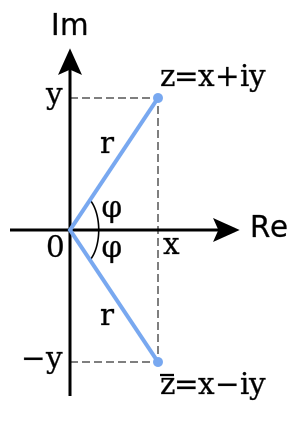
\includegraphics[width=0.9\textwidth]{images/complex.pdf}
\caption{The complex plane, taken from Wikimedia}
\end{figure}
\end{column}
\end{columns}
\end{frame}
\begin{frame}[label={sec:orgfb624d1}]{Introduction}
\begin{itemize}
\item Some familiar coordinate transformations (each with its own natural ``frame''
of vectors)
are
\end{itemize}
\begin{columns}
\begin{column}{0.4\columnwidth}
\begin{block}{Cartesian coordinates}
\begin{itemize}
\item Coordinate: \((x, y, z)\)
\item Frame : \(\hat{\gv{e}_x}, \hat{\gv{e}_y}, \hat{\gv{e}_z}\)
\end{itemize}
\end{block}
\end{column}
\begin{column}{0.6\columnwidth}
\begin{figure}[htbp]
\centering
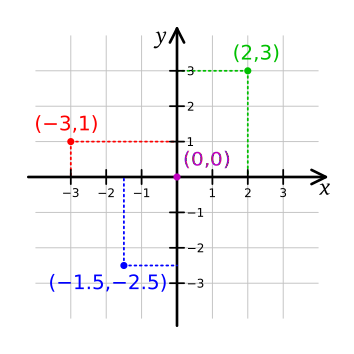
\includegraphics[width=0.8\textwidth]{images/cartesian.pdf}
\caption{Cartesian coordinate system, Wikimedia}
\end{figure}
\end{column}
\end{columns}
\end{frame}
\begin{frame}[label={sec:orgf19aa83}]{Introduction}
\begin{columns}
\begin{column}{0.4\columnwidth}
\begin{block}{Cylindrical coordinates}
\begin{itemize}
\item Coordinate: \((\rho, \phi, z)\)
\item Frame : \(\hat{\gv{e}_\rho}, \hat{\gv{e}_\phi}, \hat{\gv{e}_z}\)
\end{itemize}
\begin{figure}[htbp]
\centering
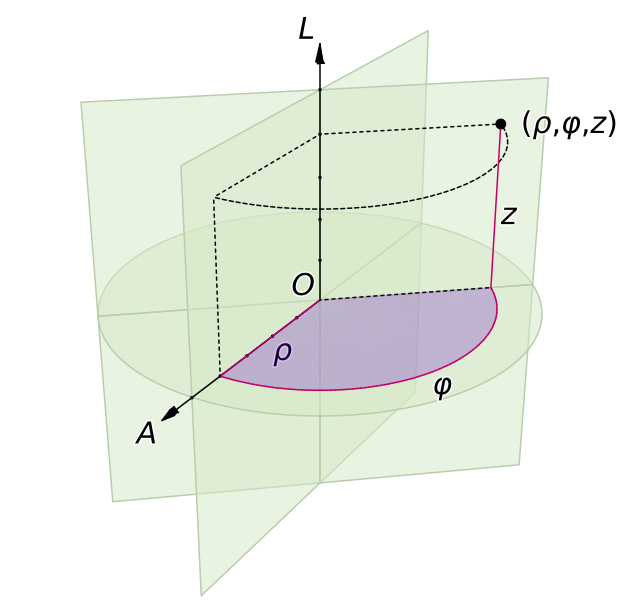
\includegraphics[height=0.8\textwidth]{images/cylindrical.pdf}
\caption{Cylindrical coordinate system, Wikimedia}
\end{figure}
\end{block}
\end{column}

\begin{column}{0.4\columnwidth}
\begin{block}{Spherical coordinates}
\begin{itemize}
\item Coordinate: \((r, \theta, \phi)\)
\item Frame : \(\hat{\gv{e}_r}, \hat{\gv{e}_\theta}, \hat{\gv{e}_\phi}\)
\end{itemize}

\begin{figure}[htbp]
\centering
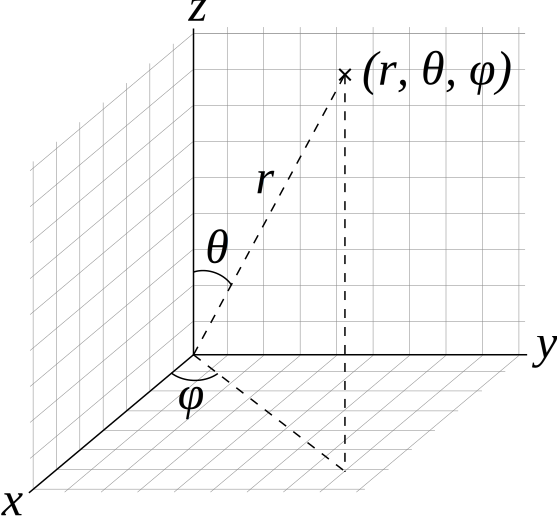
\includegraphics[height=0.8\textwidth]{images/spherical.pdf}
\caption{Spherical coordinate system, Wikimedia}
\end{figure}
\end{block}
\end{column}
\end{columns}
\end{frame}
\begin{frame}[label={sec:org2e742ab}]{Introduction}
\begin{block}{Choice of coordinate system}
\begin{itemize}
\item We represent entities (points, vectors etc.) in the \emph{cartesian coordinate
system}, considering only Euclidean geometry
\end{itemize}
\end{block}
\begin{block}{Why?}
\begin{itemize}
\item To use certain \alert{affine} transformations
\end{itemize}
\end{block}
\begin{definition}[Affine transformations]
\begin{itemize}
\item any function between \emph{affine spaces} which preserves points, straight lines and planes
\item Examples: translation, scaling, similarity transformation,
reflection, rotation, etc. and their compositions
\end{itemize}
\end{definition}
\end{frame}
\begin{frame}[label={sec:orga59020e}]{Affine transformations}
\begin{theorem}[Affine \(\leftrightarrow\) Linear]
If \(\mathcal{X}\) and \(\mathcal{Y}\) are affine spaces, then every affine transformation
\(f\colon \mathcal{X}\to \mathcal{Y}\) is of the form \(\gv{x}\mapsto
	\bv{M}\gv{x}+\gv{b}\) where \(\bv{M}\) is a linear transformation on the
space \(\mathcal{X}\),  \(\gv{x}\) is a vector in \(\mathcal{X}\), and \(\gv{b}\) is a vector in \(\mathcal{Y}\).
\end{theorem}
\end{frame}

\begin{frame}[label={sec:org608a864}]{Affine transformations : Examples}
\begin{block}{Translations ( \(\bv{M} = \bv{0}\) and \(\gv{b} \neq \gv{0}\) )}
\begin{figure}[htbp]
\centering

\includegraphics[width=0.4\textwidth]{images/translate.pdf}
\caption{Translation of entities, Wikimedia, CC4.0}
\end{figure}
\end{block}
\begin{block}{Translation \alert{DEMO}}
\end{block}
\end{frame}
\begin{frame}[label={sec:org100fc57}]{Linear transformations}
\begin{block}{Difference b/w linear and affine trans.}
\begin{itemize}
\item Most of our interest lies in modeling soft filaments, for which we will be
using only \emph{linear transformations}
\item In linear transformations, \(\gv{b} \equiv \gv{0}\) for vector spaces \(\mathcal{X}\) and \(\mathcal{Y}\)
\item We lose the ability to translate entities using linear transformations (
zero must map to zero by definition)
\end{itemize}
\end{block}
\end{frame}
\begin{frame}[label={sec:org6c85e07}]{But what are linear transformations?}
\begin{itemize}
\item We loosely define a linear transformation \(\gv{x} \to \bv{M}\gv{x}\) by a \emph{matrix}
( \(\bv{M}\) ) that acts on the vector \(\gv{x}\)
\item Check out the Wikipedia page on \href{https://en.wikipedia.org/wiki/Matrix\_(mathematics)}{matrices} and \href{https://en.wikipedia.org/wiki/Rotation\_matrix}{matrix classes} to see why they
(matrices and linear transformations) are considered important.
\end{itemize}
\end{frame}
\begin{frame}[label={sec:orgcf8c655}]{Linear transformations : Examples\footnote{All examples from Wikipedia found in \href{https://en.wikipedia.org/wiki/Affine\_transformation\#Image\_transformation}{article ``Affine transformation''
under section ``Image transformation''} and assume origin at the center of image}}
\begin{columns}
\begin{column}{0.5\columnwidth}
\begin{block}{Identity}
\[ \bv{M} = \begin{bmatrix}1&0&0\\0&1&0\\0&0&1\end{bmatrix} \]
\begin{center}
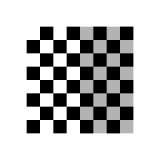
\includegraphics[height=0.8\textwidth]{images/ch_id.pdf}
\end{center}
\end{block}
\end{column}
\begin{column}{0.5\columnwidth}
\begin{block}{Reflection}
\[ \bv{M} =\begin{bmatrix}-1&0&0\\0&1&0\\0&0&1\end{bmatrix} \]
\begin{center}
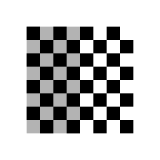
\includegraphics[height=0.8\textwidth]{images/ch_ref.pdf}
\end{center}
\end{block}
\end{column}
\end{columns}
\end{frame}

\begin{frame}[label={sec:orgcbec8a8}]{Linear transformations : Examples}
\begin{columns}
\begin{column}{0.5\columnwidth}
\begin{block}{Scale}
\[ \bv{M} =\begin{bmatrix}c_{x}=2&0&0\\0&c_{y}=1&0\\0&0&1\end{bmatrix} \]
\begin{center}
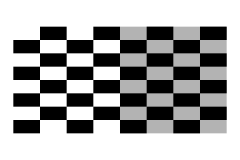
\includegraphics[height=0.8\textwidth]{images/ch_sc.pdf}
\end{center}
\end{block}
\end{column}
\begin{column}{0.5\columnwidth}
\begin{block}{Shear}
\[ \bv{M} =\begin{bmatrix}1&c_{x}=0.5&0\\c_{y}=0&1&0\\0&0&1\end{bmatrix}\]
\begin{center}
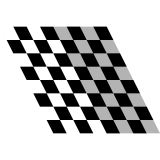
\includegraphics[height=0.8\textwidth]{images/ch_sh.pdf}
\end{center}
\end{block}
\end{column}
\end{columns}
\end{frame}

\begin{frame}[label={sec:orgc8ce753}]{Linear transformations : Examples}
\begin{block}{Rotation}
\begin{center}
\spot<2>{\( \bv{M} =\begin{bmatrix}\cos(\theta )&\sin(\theta )&0\\-\sin(\theta
 )&\cos(\theta )&0\\0&0&1\end{bmatrix} \text{with } \theta = \frac{\pi}{6}\)}
\end{center}

\begin{center}
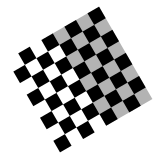
\includegraphics[height=0.5\textwidth]{images/ch_rot.pdf}
\end{center}
\end{block}
\end{frame}
\begin{frame}[label={sec:org109d21c}]{Rotations (includes reflections)}
\begin{itemize}
\item Generates new unit vectors, fundamentally changing the directions
(eigenvectors) of further transformations
\item Does not scale the entity under consideration ( \(\abs{\lambda} \equiv  1\), more on this later\ldots{})
\end{itemize}
\end{frame}
\begin{frame}[label={sec:org19cc3a3}]{Frame rotations in two--dimensions}
Consider
\begin{figure}[htbp]
\centering
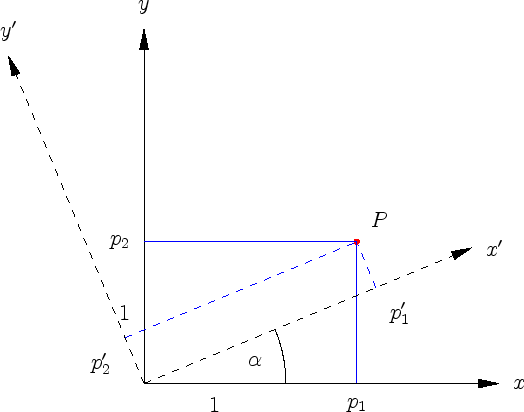
\includegraphics[width=0.45\textwidth]{images/cartesian_rotation.png}
\caption{Rotation in two dimensions}
\end{figure}

\[ \begin{bmatrix} x^\prime \\ y^\prime \end{bmatrix}
   = \underbrace{\begin{bmatrix}\cos(\alpha )&\sin(\alpha )\\ -\sin(\alpha
   )&\cos(\alpha )\end{bmatrix}}_{\bv{R}} \begin{bmatrix} x\\ y\end{bmatrix}\]
\end{frame}
\begin{frame}[label={sec:orga4ab53a}]{Inverse rotations in two--dimensions}
Now consider the same picture, but we want to obtain \([x,y]^T\) from \([
   x^\prime, y^\prime ]^T\) (the other way around).

\begin{itemize}
\item Physically, this is just a rotation of \(- \alpha\) counter-clockwise (or
\(\alpha\) clockwise). That means
\end{itemize}
\[ \begin{bmatrix} x\\ y\end{bmatrix}
   = \begin{bmatrix}\cos(\alpha )& -\sin(\alpha )\\ \sin(\alpha
   )& \cos(\alpha )\end{bmatrix}  \begin{bmatrix} x^\prime \\ y^\prime
   \end{bmatrix} \]
\begin{itemize}
\item Mathematically, if \(\gv{x}^\prime= \bv{R} \gv{x}\), then we know \(\gv{x}= \bv{R}^{-1} \gv{x}^\prime\), provided \(\bv{R}^{-1}\) exists
(which does).
\item Then notice that
\end{itemize}
\[ \bv{R}^{-1} = \begin{bmatrix}\cos(\alpha )& -\sin(\alpha )\\ \sin(\alpha
   )& \cos(\alpha )\end{bmatrix}  = \bv{R}^T ! \]
\begin{itemize}
\item We will see later why holds for \alert{all} rotation matrices\ldots{}
\end{itemize}
\end{frame}
\begin{frame}[label={sec:orgecf4926}]{Frame rotations in three--dimensions}
\begin{figure}[htbp]
\centering
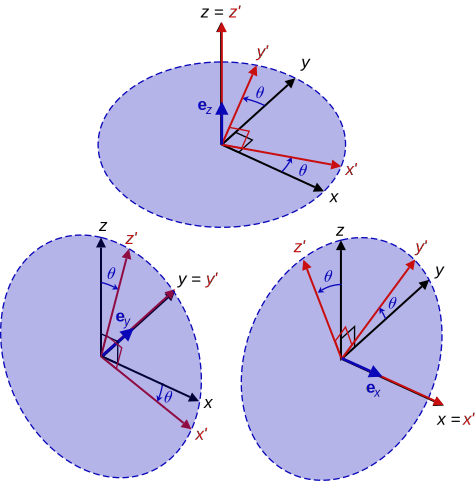
\includegraphics[width=0.45\textwidth]{images/cartesian_rot_3D.pdf}
\caption{Rotation in three dimensions, Wikimedia CC1.0}
\end{figure}
is a natural extension of 2D results\ldots{}
\end{frame}
\begin{frame}[label={sec:orgbc66b2c}]{Beware!}
\begin{block}{Be wary about alias (passive) or alibi (active) transformations}
\end{block}
\begin{columns}
\begin{column}{0.55\columnwidth}
\begin{definition}[Alias transformations]
Involves rotation of the coordinate system or frame
(change in basis)
\end{definition}
\begin{definition}[Alibi transformations]
Involves rotation of the entities within the same
frame (change in entity)
\end{definition}
\end{column}
\begin{column}{0.5\columnwidth}
\begin{figure}[htbp]
\centering
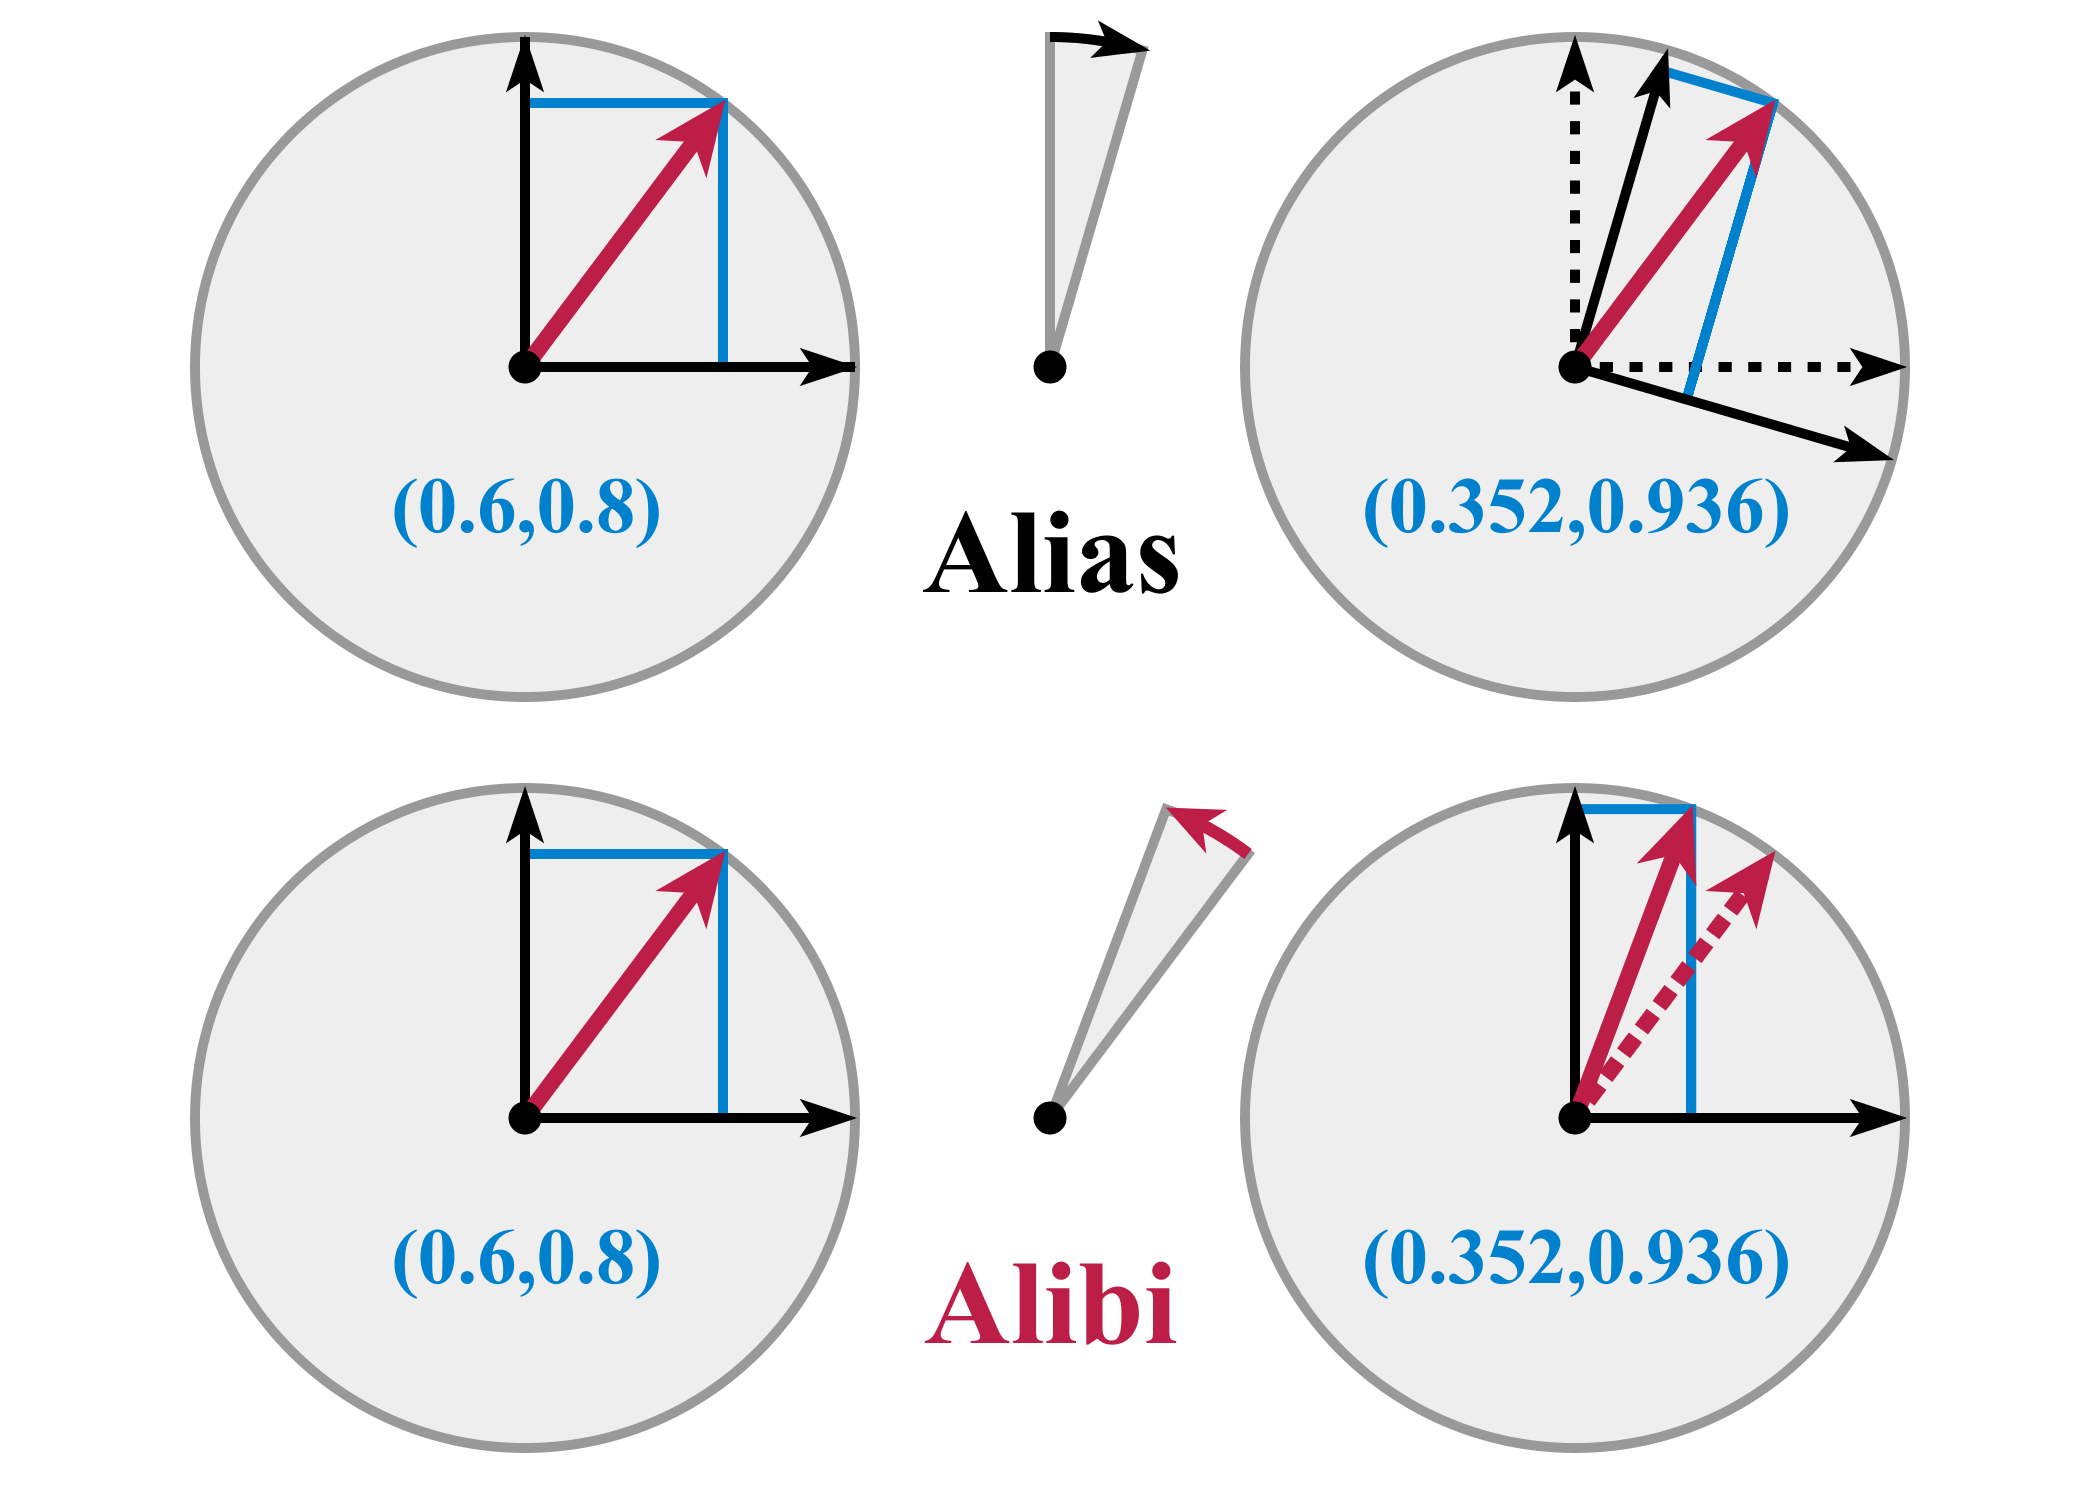
\includegraphics[width=1.00\textwidth]{images/alias_alibi.png}
\caption{Alias-Alibi transformations, Wikimedia CC3.0}
\end{figure}
\end{column}
\end{columns}
Both are equally valid ways of representing rotations---in this class
however, we focus on alias transformations.
\note{:B\_note:
\begin{itemize}
\item Affirm that the entity does not matter. Show this for a vector or a point.
Beauty of affine transformations.
\item To change the formulas for passive rotations (or find reverse active
rotation), transpose the matrices (then each matrix transforms the initial
coordinates of a vector remaining fixed to the coordinates of the same
vector measured in the rotated reference system; same rotation axis, same
angles, but now the coordinate system rotates, rather than the vector).
\end{itemize}}
\end{frame}
\begin{frame}[label={sec:orgc90fd97}]{Difference in perspectives\footnote{\href{https://iopscience.iop.org/book/978-0-7503-1454-1}{Rotation, Reflection, and Frame Changes---Orthogonal tensors in computational engineering mechanics, RM Brannon, IOP Publishing 2018}}}
\begin{quotation} %% :B\_quotation:
`` Analyzing rotation demands awareness of your desired perspective. You can rotate an object, while you stay still, or you can keep the object
fixed while you rotate yourself. It is important to be aware of which of these
perspectives applies for your problem of interest. The distinction between
these fundamentally different transformations goes beyond one being the
same as the other with an opposite rotation angle. ''
\end{quotation}
\end{frame}
\begin{frame}[label={sec:orgdfac8aa}]{Frame rotation as a change in basis}
\begin{block}{More concretely}
If \(\mathcal{B}\) and \(\mathcal{B}^\prime\) are two (different) bases
\(\in \mathbb{R}^n\)
\begin{itemize}
\item Alibi : Change in entity \([\gv{p}]_{\mathcal{B}} \to
      [\gv{p}^\prime]_{\mathcal{B}}\) given by
\end{itemize}
\[ [\gv{p}^\prime]_{\mathcal{B}} = [\bv{M}]_{\mathcal{B} \to \mathcal{B}}
  [\gv{p}]_{\mathcal{B}} \]
\begin{itemize}
\item Alias : Change in basis \([\gv{p}]_{\mathcal{B}} \to
      [\gv{p}]_{\mathcal{B}^\prime}\)
\end{itemize}
\[ [\gv{p}]_{\mathcal{B}^\prime} = [\bv{M}]_{\mathcal{B} \to \mathcal{B}^\prime}
  [\gv{p}]_{\mathcal{B}} \]
\begin{itemize}
\item In our soft filament framework, \(\mathcal{B}^\prime \equiv \mathcal{L}\) and  \(\mathcal{B} \equiv\) lab frame. \(\bv{Q}\) is then the
basis transformation matrix (corresponding to pure rotation of the
orthonormal bases)
\end{itemize}
\end{block}
\end{frame}
\begin{frame}[label={sec:org0e99f12}]{Frame rotation---example}
\begin{columns}
\begin{column}{0.5\columnwidth}
\tdplotsetmaincoords{60}{100}
\begin{center}
 \begin{tikzpicture}[scale=2, tdplot_main_coords]
 \draw[thick,->, color=scarlet] (0,0,0) -- (1,0,0) node[anchor=north east]{$x$};
 \draw[thick,->, color=shamrockgreen] (0,0,0) -- (0,1,0) node[anchor=north west]{$y$};
 \draw[thick,->, color=royalblue] (0,0,0) -- (0,0,1) node[anchor=south]{$z$};
 \end{tikzpicture}
\end{center}
\end{column}
\begin{column}{0.5\columnwidth}
\tdplotsetmaincoords{60}{100}
\begin{center}
 \begin{tikzpicture}[scale=2, tdplot_main_coords]
 \draw[dashed,->,line width= 1.1pt] (0,0,0) -- (1,0,0) node[anchor=north east]{$x$};
 \draw[dashed,->,line width= 1.1pt] (0,0,0) -- (0,1,0) node[anchor=north west]{$y$};
 \draw[dashed,->,line width= 1.1pt] (0,0,0) -- (0,0,1) node[anchor=south west]{$z$};

 \coordinate (Shift) at (0,0,0);
 \tdplotsetrotatedcoords{0}{0}{90}
 \tdplotsetrotatedcoordsorigin{(Shift)}

 \draw[thick,color=scarlet,tdplot_rotated_coords,->] (0,0,0)
 -- (1,0,0) node[anchor=south east]{$x’$};
 \draw[thick,color=shamrockgreen,tdplot_rotated_coords,->] (0,0,0)
 -- (0,1,0) node[anchor=west]{$y’$};
 \draw[thick,color=royalblue,tdplot_rotated_coords,->] (0,0,0)
 -- (0,0,1) node[anchor=south east]{$z’$};
 \end{tikzpicture}
\end{center}
\end{column}
\end{columns}
\begin{itemize}
\item Represent \((x-y-z)\) axis with a basis \(\mathcal{E}\) of unit vectors \(\hat{\gv{e}_1}, \hat{\gv{e}_2}, \hat{\gv{e}_3}\)
\item Represent \((x'-y'-z')\) axis with a basis \(\mathcal{D}\) of unit vectors \(\hat{\gv{d}_1}, \hat{\gv{d}_2}, \hat{\gv{d}_3}\)
\item \(\mathcal{E} \to \mathcal{D}\)?
\item Note : rotation of \(\ang{90}\) about an invariant \(z' = z\) axis
\end{itemize}
\end{frame}
\begin{frame}[label={sec:orgee92ec1}]{Frame rotation---example contd.}
\[ {\begin{bmatrix} x^\prime \\ y^\prime \\ z^\prime\end{bmatrix}} =
  \spot{[\bv{M}]_{\mathcal{E} \to \mathcal{D}}}
  {\begin{bmatrix} x \\ y \\ z \end{bmatrix}}
  \]
\begin{itemize}
\item We begin by noticing that \(\begin{bmatrix} x^\prime , y^\prime , z^\prime
     \end{bmatrix} = \begin{bmatrix} y , -x , z \end{bmatrix}\) (from figure). Then
\end{itemize}
\[ {\begin{bmatrix} x^\prime \\ y^\prime \\ z^\prime\end{bmatrix}} =
  {\begin{bmatrix} 0 & 1 & 0 \\ -1 & 0 & 0 \\ 0 & 0 & 1 \end{bmatrix}}
  {\begin{bmatrix} x \\ y \\ z \end{bmatrix}}
  \]
\[\Rightarrow {\begin{bmatrix} x^\prime \\ y^\prime \\ z^\prime\end{bmatrix}} =
  {\begin{bmatrix} \cos(\ang{90}) & \sin(\ang{90}) & 0 \\ -\sin(\ang{90}) &
  \cos(\ang{90}) & 0 \\ 0 & 0 & 1 \end{bmatrix}}
  {\begin{bmatrix} x \\ y \\ z \end{bmatrix}}
  \]
\end{frame}
\begin{frame}[label={sec:org84493d7}]{Generalizing frame rotations as a basis change}
\begin{itemize}
\item But also notice with the given bases that
\end{itemize}
\[{\begin{bmatrix} x^\prime \\ y^\prime \\ z^\prime\end{bmatrix}_{\mathcal{D}}} =
  \spot<2>{
  \underbrace{\begin{bmatrix}
  \hat{\gv{d}}_1 \cdot \hat{\gv{e}}_1 & \hat{\gv{d}}_1 \cdot
  \hat{\gv{e}}_2 & \hat{\gv{d}}_1 \cdot \hat{\gv{e}}_3 \\
  \hat{\gv{d}}_2 \cdot \hat{\gv{e}}_1 & \hat{\gv{d}}_2 \cdot
  \hat{\gv{e}}_2 & \hat{\gv{d}}_2 \cdot \hat{\gv{e}}_3 \\
  \hat{\gv{d}}_3 \cdot \hat{\gv{e}}_1 & \hat{\gv{d}}_3 \cdot
  \hat{\gv{e}}_2 & \hat{\gv{d}}_3 \cdot \hat{\gv{e}}_3
  \end{bmatrix}}_{[\bv{M}]_{\mathcal{E} \to \mathcal{D}}, \text{ independent of
  } \mathbf{x}}
  }
  {\begin{bmatrix} x \\ y \\ z \end{bmatrix}_{\mathcal{E}}}
  \]
\begin{block}<2->{Soft filament framework}
\begin{itemize}
\item Describe lab frame, \(\mathcal{E}\), by natural bases \(\hat{i}, \hat{j}, \hat{k}\).
\item Describe material (Lagrangian) frame, \(\mathcal{D}\), by orthonormal
vectors \(\hat{\gv{d}_1}, \hat{\gv{d}_2}, \hat{\gv{d}_3}\) (coordinates wrt
natural bases). Then
\end{itemize}
\[{\begin{bmatrix} x_{\mathcal{L}} \\ y_{\mathcal{L}} \\ z_{\mathcal{L}} \end{bmatrix}_{\mathcal{D}}} =
	 \underbrace{\begin{bmatrix}
	 \mbox{------}~\hat{\gv{d}}_1~\mbox{------} \\
	 \mbox{------}~\hat{\gv{d}}_2~\mbox{------} \\
	 \mbox{------}~\hat{\gv{d}}_3~\mbox{------} \\
	 \end{bmatrix}}_{\bv{Q}}
	 {\begin{bmatrix} x \\ y \\ z \end{bmatrix}_{\mathcal{E}}}
   \]
\end{block}
\end{frame}
\begin{frame}[label={sec:org4de8675}]{Generalizing frame rotations as a basis change}
 Taking it one step further we arrive at the conclusion,
\[
	\underbrace{\begin{bmatrix}
	\mbox{|} & \mbox{|}& \mbox{|}\\
	\hat{\gv{d}_1} & \hat{\gv{d}_2} & \hat{\gv{d}_3} \\
	\mbox{|} & \mbox{|}& \mbox{|}\\
	\end{bmatrix}}_{\bv{Q}^{-1} = \bv{Q}^T}
	{\begin{bmatrix} x_{\mathcal{L}} \\ y_{\mathcal{L}} \\ z_{\mathcal{L}}
	\end{bmatrix}}
	=
	{\begin{bmatrix}1 & 0 & 0 \\ 0 & 1 & 0 \\0 & 0& 1\end{bmatrix}}
	{\begin{bmatrix} x \\ y \\ z \end{bmatrix}}
  \]

\[
  \Rightarrow x_{\mathcal{L}}\hat{\gv{d}_1} + y_{\mathcal{L}}\hat{\gv{d}_2} +
  z_{\mathcal{L}}\hat{\gv{d}_3} = x\hat{i} + y\hat{j} + z\hat{k} = \gv{x} !
  \]
\end{frame}
\begin{frame}[label={sec:org5478d69}]{Implementation of rotation as bases change}
\begin{itemize}
\item We have seen that the action of frame rotation matrices correspond to a
bases change operation
\item Let's implement these operations in our framework
\[ R_{x}(\theta)={\begin{bmatrix}1&0&0\\0&\cos \theta &\sin \theta
     \\0&-\sin \theta &\cos \theta \\\end{bmatrix}}\]

\[ R_{y}(\theta)={\begin{bmatrix}\cos \theta & 0 & -\sin \theta\\
	 0&1&0 \\ \sin\theta & 0 & \cos \theta \\\end{bmatrix}} \]

\[R_{z}(\theta)={\begin{bmatrix}\cos \theta &\sin \theta &0\\-\sin
	 \theta &\cos\theta &0\\0&0&1\\\end{bmatrix}} \]
\item \alert{DEMO}
\end{itemize}
\end{frame}
\begin{frame}[label={sec:org99d4804}]{But what about arbitrary rotations?}
\begin{itemize}
\item Rotations about arbitrary axes with arbitrary angles?
\end{itemize}
\begin{columns}
\begin{column}{0.6\columnwidth}
\begin{itemize}
\item Can we do compositions?
\begin{itemize}
\item \alert{Yes}, but not that intutive (means of rotation, intrinsic/extrinsic)
\item Not commutative (order matters) usually
\end{itemize}
\end{itemize}
\end{column}
\begin{column}{0.3\columnwidth}
\begin{center}
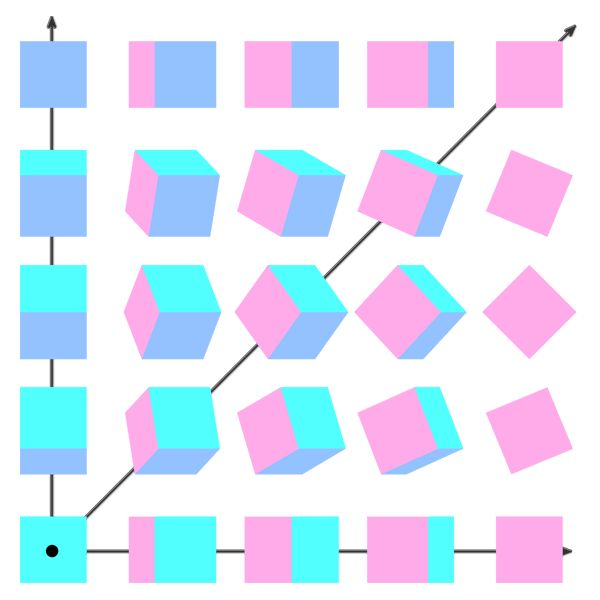
\includegraphics[width=0.80\textwidth]{images/rotated_cube.jpeg}
\end{center}
\end{column}
\end{columns}
\begin{itemize}
\item Becomes even more complicated when we have frames depending on one another
\begin{itemize}
\item But not a bad idea---robotics\footnote{\href{https://www.mecademic.com/resources/Euler-angles/Euler-angles}{Mecademic Euler rotations}}
\end{itemize}
\item \alert{Idea}: If we know the linear bases transformation, we don't need to worry
about compositions etc.
\end{itemize}
\note{:B\_note:
\begin{itemize}
\item Mention that some means of rotation like quarternions are better suited,
but require more math and understanding.
\end{itemize}}
\end{frame}
\begin{frame}[label={sec:org302ae72}]{Let's reconsider what we know}
\begin{itemize}
\item We know why \(\gv{x}_{\mathcal{L}} = \bv{Q}\gv{x}\)
\item But\ldots{}
\begin{itemize}
\item Do we know \(\bv{Q}\) ?
\begin{itemize}
\item We need the basis \(\hat{\gv{d}}_j\)
\end{itemize}
\item Do we know \(\hat{\gv{d}}_j\)?
\begin{itemize}
\item \alert{No}
\end{itemize}
\end{itemize}
\item We seek ways to obtain this basis \(\gv{d}\).
\item We will see that we require some properties on \(\gv{d}\) to make \(\bv{Q}\) effect a rotation.
\end{itemize}
\end{frame}
\begin{frame}[label={sec:org632ebf0}]{Obtaining \(\gv{d}\) : Options}
\begin{itemize}
\item
\end{itemize}
\end{frame}
\begin{frame}[label={sec:org1fde7a6}]{Rotations about fixed axis : Euler angles}
\end{frame}
\begin{frame}[label={sec:org0b3427e}]{Rotation using Euler angles : Implementation}
\end{frame}
\begin{frame}[label={sec:orgaef4d6a}]{Rotations using Euler angles: compositions}
\begin{itemize}
\item Show Rz * Ry * Rx
\item Put formula for the same here
\item
\end{itemize}
\end{frame}
\begin{frame}[label={sec:org90aa6d1}]{Rotations using Euler angles: compositions contd.}
\begin{itemize}
\item Is it commutative (does the order matter)
\end{itemize}
\begin{itemize}
\item Extrinsic or Intrinsic
\end{itemize}
\end{frame}
\begin{frame}[label={sec:orge34d5d2}]{Drawbacks of only using Euler-angle based rotation}
Not as intutive as only one axes. Althogugh it is possible.
\end{frame}
\begin{frame}[label={sec:org8a9c02c}]{Other options}
\alert{*
*}
\end{frame}
\end{document}
